\documentclass[11pt, a4paper]{article}
\usepackage{pdfpages}
\usepackage{parallel}
\usepackage[T2A]{fontenc}
%\usepackage{ucs}
\usepackage[utf8]{inputenc}
\usepackage[english,russian]{babel}
\usepackage{hyperref}
\usepackage{rotating}
\usepackage[inner=2cm,top=1.8cm,outer=2cm,bottom=2.3cm,nohead]{geometry}
%\usepackage{listings}
\usepackage{graphicx}
\usepackage{wrapfig}
\usepackage{longtable}
\usepackage{indentfirst}
\usepackage{array}
\usepackage{tikzsymbols}
\usepackage{soul}
\usepackage[ruled,vlined]{algorithm2e}
\usepackage{qrcode}
\counterwithout{figure}{section} 

\usepackage{url}
\makeatletter
\g@addto@macro{\UrlBreaks}{\UrlOrds}
\makeatother

\newcolumntype{P}[1]{>{\raggedright\arraybackslash}p{#1}}
\frenchspacing
%\usepackage{fixltx2e} %text sub- and superscripts
\usepackage{icomma} % коскі ў матэматычным рэжыме
%\PreloadUnicodePage{4}

\newcommand{\longpage}{\enlargethispage{\baselineskip}}
\newcommand{\shortpage}{\enlargethispage{-\baselineskip}}

\def\switchlang#1{\expandafter\csname switchlang#1\endcsname}
\def\switchlangbe{
\let\saverefname=\refname%
\def\refname{Літаратура}%
\def\figurename{Іл.}%
}
\def\switchlangru{
\let\saverefname=\refname%
\let\savefigurename=\figurename%
\def\refname{Литература}%
\def\figurename{Рис.}%
}
\def\switchlangen{
\let\saverefname=\refname%
\def\refname{References}%
\def\figurename{Fig.}%
}

\hyphenation{admi-ni-stra-tive}
\hyphenation{ex-pe-ri-ence}
\hyphenation{fle-xi-bi-li-ty}
\hyphenation{Py-thon}
\hyphenation{ma-the-ma-ti-cal}
\hyphenation{re-ported}
\hyphenation{imp-le-menta-tions}
\hyphenation{pro-vides}
\hyphenation{en-gi-neering}
\hyphenation{com-pa-ti-bi-li-ty}
\hyphenation{im-pos-sible}
\hyphenation{desk-top}
\hyphenation{elec-tro-nic}
\hyphenation{com-pa-ny}
\hyphenation{de-ve-lop-ment}
\hyphenation{de-ve-loping}
\hyphenation{de-ve-lop}
\hyphenation{da-ta-ba-se}
\hyphenation{plat-forms}
\hyphenation{or-ga-ni-za-tion}
\hyphenation{pro-gramming}
\hyphenation{in-stru-ments}
\hyphenation{Li-nux}
\hyphenation{sour-ce}
\hyphenation{en-vi-ron-ment}
\hyphenation{Te-le-pathy}
\hyphenation{Li-nux-ov-ka}
\hyphenation{Open-BSD}
\hyphenation{Free-BSD}
\hyphenation{men-ti-on-ed}
\hyphenation{app-li-ca-tion}

\def\progref!#1!{\texttt{#1}}
\renewcommand{\arraystretch}{2} %Іначай формулы ў матрыцы зліпаюцца з лініямі
\usepackage{array}

\def\interview #1 (#2), #3, #4, #5\par{

\section[#1, #3, #4]{#1 -- #3, #4}
\def\qname{LVEE}
\def\aname{#1}
\def\q ##1\par{{\noindent \bf \qname: ##1 }\par}
\def\a{{\noindent \bf \aname: } \def\qname{L}\def\aname{#2}}
}

\def\interview* #1 (#2), #3, #4, #5\par{

\section*{#1\\{\small\rm #3, #4. #5}}
\ifx\ParallelWhichBox\undefined%
    \addcontentsline{toc}{section}{#1, #3, #4}%
\else%
\ifnum\ParallelWhichBox=0%
    \addcontentsline{toc}{section}{#1, #3, #4}%
\fi\fi%

\def\qname{LVEE}
\def\aname{#1}
\def\q ##1\par{{\noindent \bf \qname: ##1 }\par}
\def\a{{\noindent \bf \aname: } \def\qname{L}\def\aname{#2}}
}

\newcommand{\interviewfooter}[1]{
\vskip 1em
\noindent \textit{#1}
}

\AtEndDocument{\vfill\centering \qrcode{https://github.com/fiowro/mouses/blob/main/\jobname.pdf}}

\switchlang{ru}
\begin{document}

\title{1985 "--- Vatek Color-Mouse}
\date{}
\maketitle
\selectlanguage{russian}

Мышь Vatek Color-Mouse была выпущена в продажу в 1989 году компанией Vatek USA Inc. "--- дистрибьютором компьютерного оборудования, зарегистрированным в Калифорнии годом ранее. По утверждению создателей мыши, в результате этого Vatek стала первой компанией, официально представившей на рынке мышь в многоцветном исполнении. Этот приоритет нельзя назвать бесспорным: в рекламных материалах Hawley Mouse House 1982 года красуется рисунок  Mark II X063X Mouse в десятках цветовых сочетаний. Но реально цветовых вариантов Mark II было выпущено не так уж много; кроме того, Hawley Mouse House не делала упор на многоцветность, а Vatek не только позиционировала свое изделие в этом качестве, но даже закрепила его в названии мыши. Наконец, утверждение Vatek можно понимать и буквально, в том смысле, что компания первая представила на рынке компьютерную мышь под названием <<color mouse>> (англ. <<цветная мышь>>), с чем действительно не приходится спорить.

\begin{figure}[h]
   \centering
    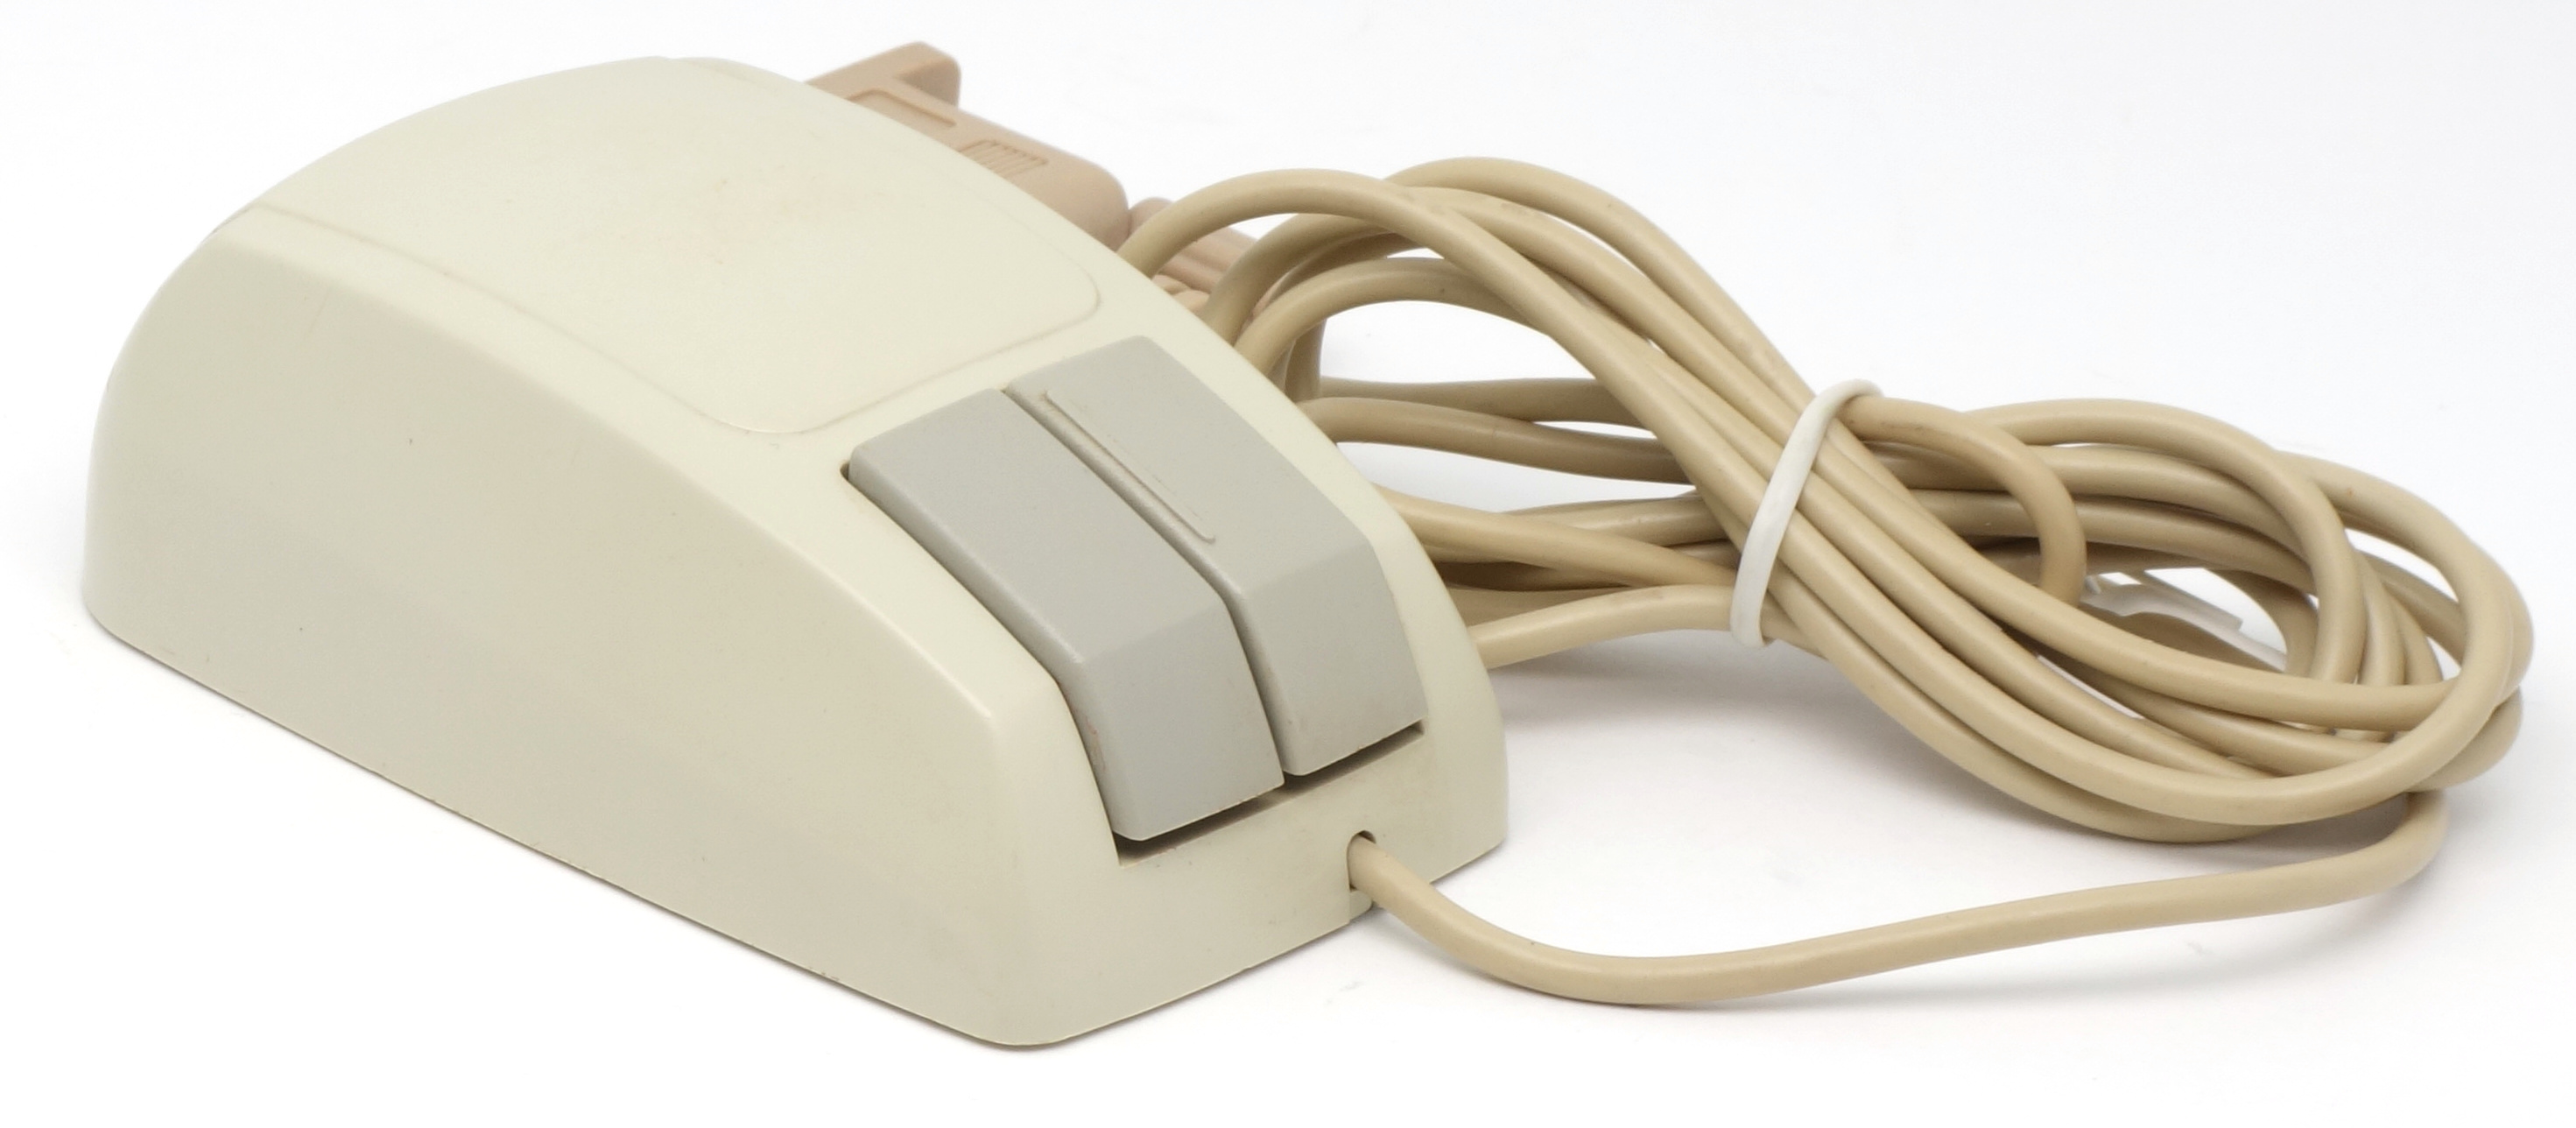
\includegraphics[scale=0.45]{1989_vatek_color_mouse/pic_30.jpg}
    \caption{Microsoft Gray-eyed Mouse}
    \label{fig:VatekColorPic}
\end{figure}

Корпус устройства изготавливался из пластика красного, зеленого, желтого или синего цвета, но иногда и из стандартного бежевого \cite{mouses}, и всегда оснащался двумя контрастными серыми кнопками. Как можно видеть (рис. \ref{fig:VatekColorPic}), данный экземпляр <<цветной>> мыши является именно бежевым.

\begin{figure}[h]
    \centering
    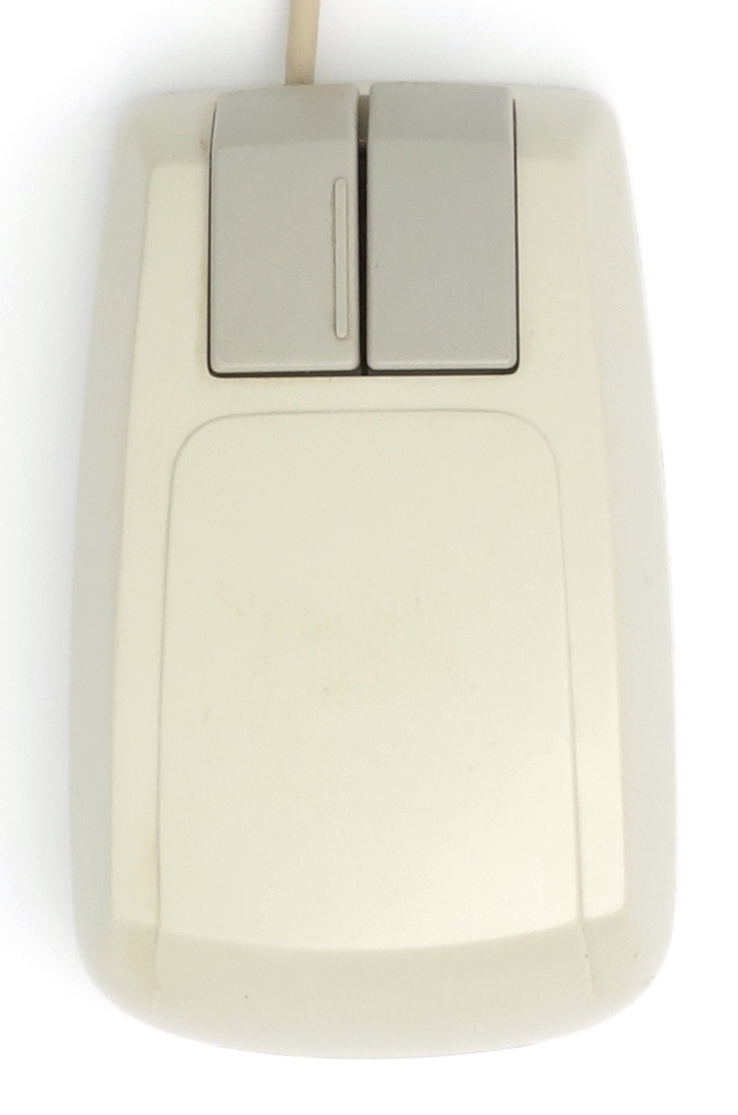
\includegraphics[scale=0.55]{1989_vatek_color_mouse/top_30.jpg}
    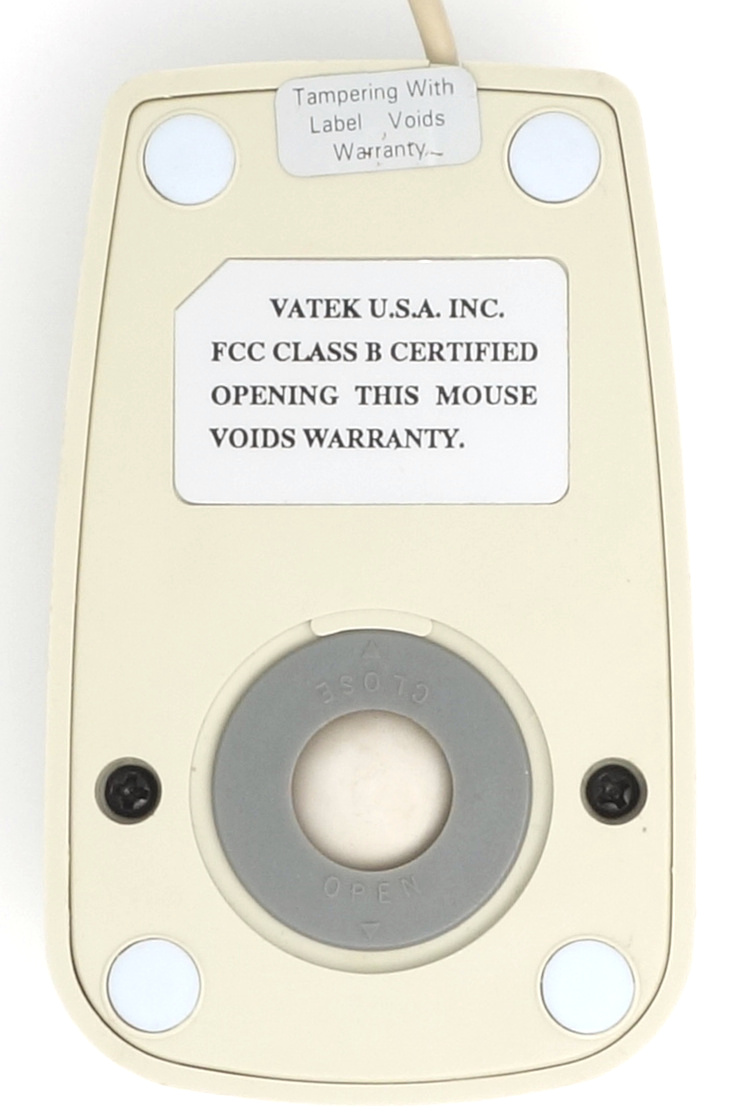
\includegraphics[scale=0.55]{1989_vatek_color_mouse/bottom_30.jpg}
    \caption{Microsoft Gray-eyed Mouse, вид сверху и снизу}
    \label{fig:VatekColorTopAndBottom}
\end{figure}

Форма мыши копирует вышедшую в 1985 году мышь Microsoft второго поколения (известную под названием <<сероглазой>> мыши из-за цвета кнопок). Верхняя часть корпуса Vatek Color-Mouse воспроизводит корпус мыши Microsoft вплоть до идентичности, за исключением более широких кнопок, смыкающихся друг с другом (рис. \ref{fig:VatekColorTopAndBottom}). При этом главная кнопка имеет продольный выступ для легкой тактильной идентификации ее края, что позаимствовано уже из третьего поколения мышей Microsoft.
Снизу можно видеть шар с резиновым покрытием, фиксирующее кольцо, сдвигаемое для извлечения шара и чистки мыши, табличку с техническими данными (упоминается, но не приведен, код FCC), а также четыре низкофиркционные накладки. Нижняя сторона уже не копирует <<сероглазую>> мышь Microsoft (а точнее, не копирует лежащий в ее основе типовой дизайн ALPS), если не считать общего силуэта и положения шара в задней части корпуса.

\begin{figure}[h]
    \centering
    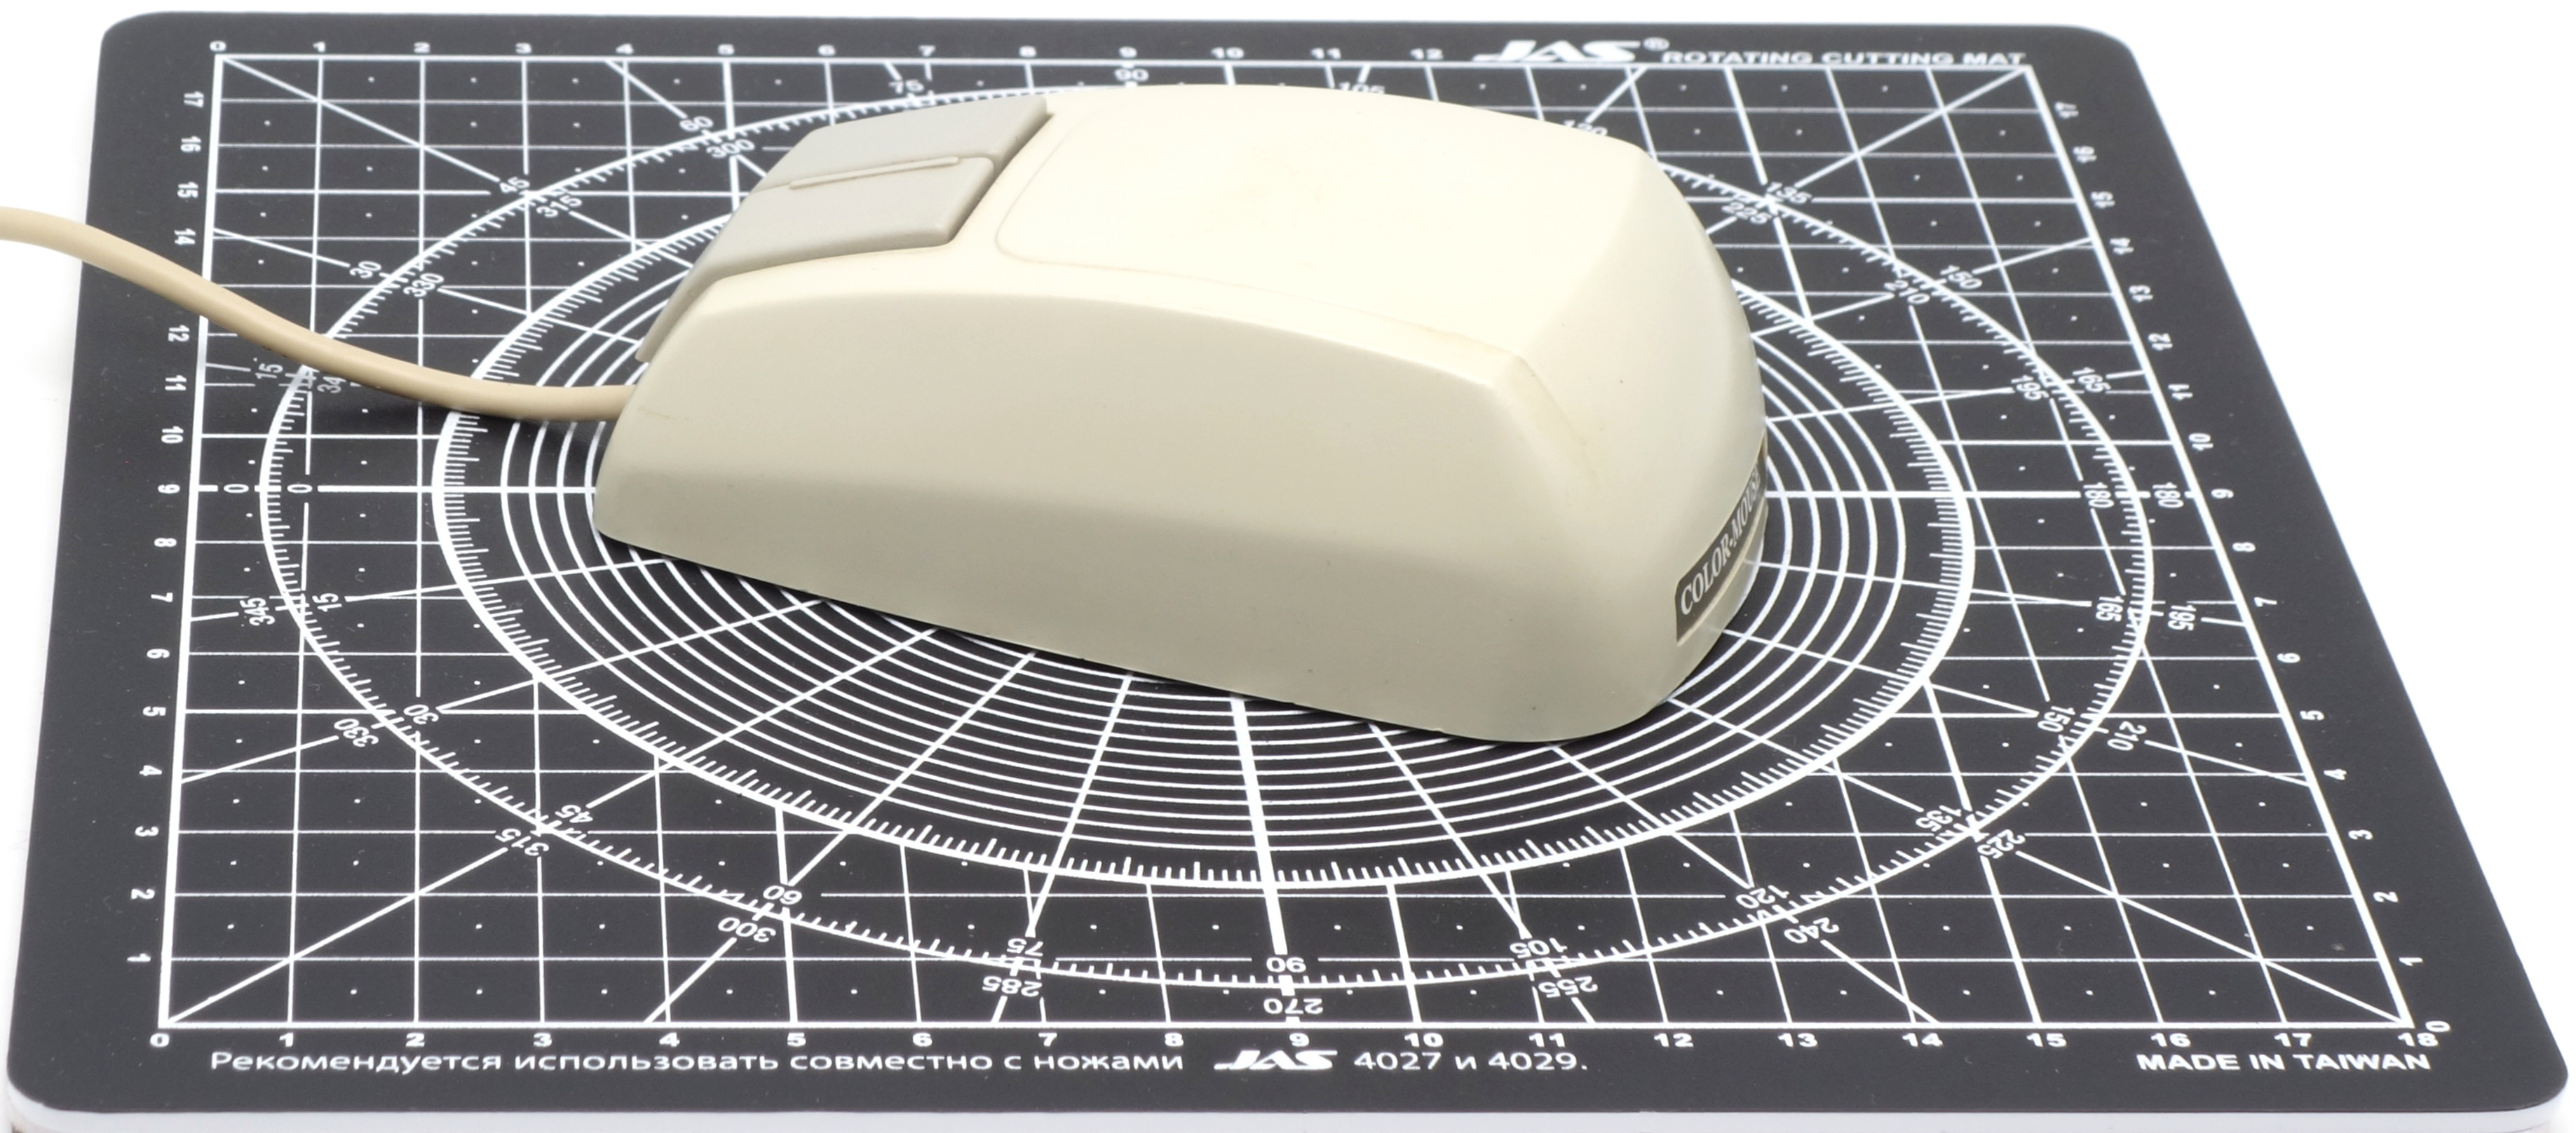
\includegraphics[scale=0.4]{1989_vatek_color_mouse/size_30.jpg}
    \caption{Microsoft Gray-eyed Mouse на размерном коврике с шагом сетки 1~см}
    \label{fig:VatekColorSize}
\end{figure}

По понятной причине размеры мыши позаимствованы у Microsoft (рис. \ref{fig:VatekColorSize}), в случае которой они определялись размерами типового узла ALPS. Помимо двухкнопочной Color-Mouse в то же время в таком же корпусе выпускался трехкнопочный вариант мыши: он продавался под различными брэндами, как известными так и нет, и различными названиями: Z-Nix Super Hi-Res Mouse, ProCorp Serial Mouse, SmarTEAM Smart Mouse и др.

Эргономика Color-Mouse также во многом повторяет особенности мыши Microsoft за счет того же самого высокого корпуса, удобного для захвата узкой ладонью, и угловых кнопок, немного отличаясь в лучшую сторону за счет того, что кнопки Vatek шире.
Такая угловая форма кнопок придумана Microsoft как логическое развитие мыши первого поколения, кнопки которой помещались на корпусе спереди и вызывали критику со стороны некоторых обозревателей из-за возможности нечаянно сдвинуть мышь, просто нажимая на них. В рекламных материалах <<сероглазой>> мыши Microsoft упоминается, что <<огибающие корпус командные кнопки спроектированы таким образом, чтобы естественно помещаться в ладони любого размера>> \cite{mouses}, но очевидно, такое двойное положение кнопок решало и проблему ошибочных перемещений, позволяя нажимать на них сверху тем, кому это удобнее (рис. \ref{fig:VatekColorHand}). Вслед за Microsoft, эта угловая форма кнопок появилась в некоторых других мышах и больше всего сходства по понятным причинам демонстрируют Vatek Сolor-Mouse и её трехкнопочный близнец, известный под именем ProCorp Serial Mouse и др.

\begin{figure}[h]
    \centering
    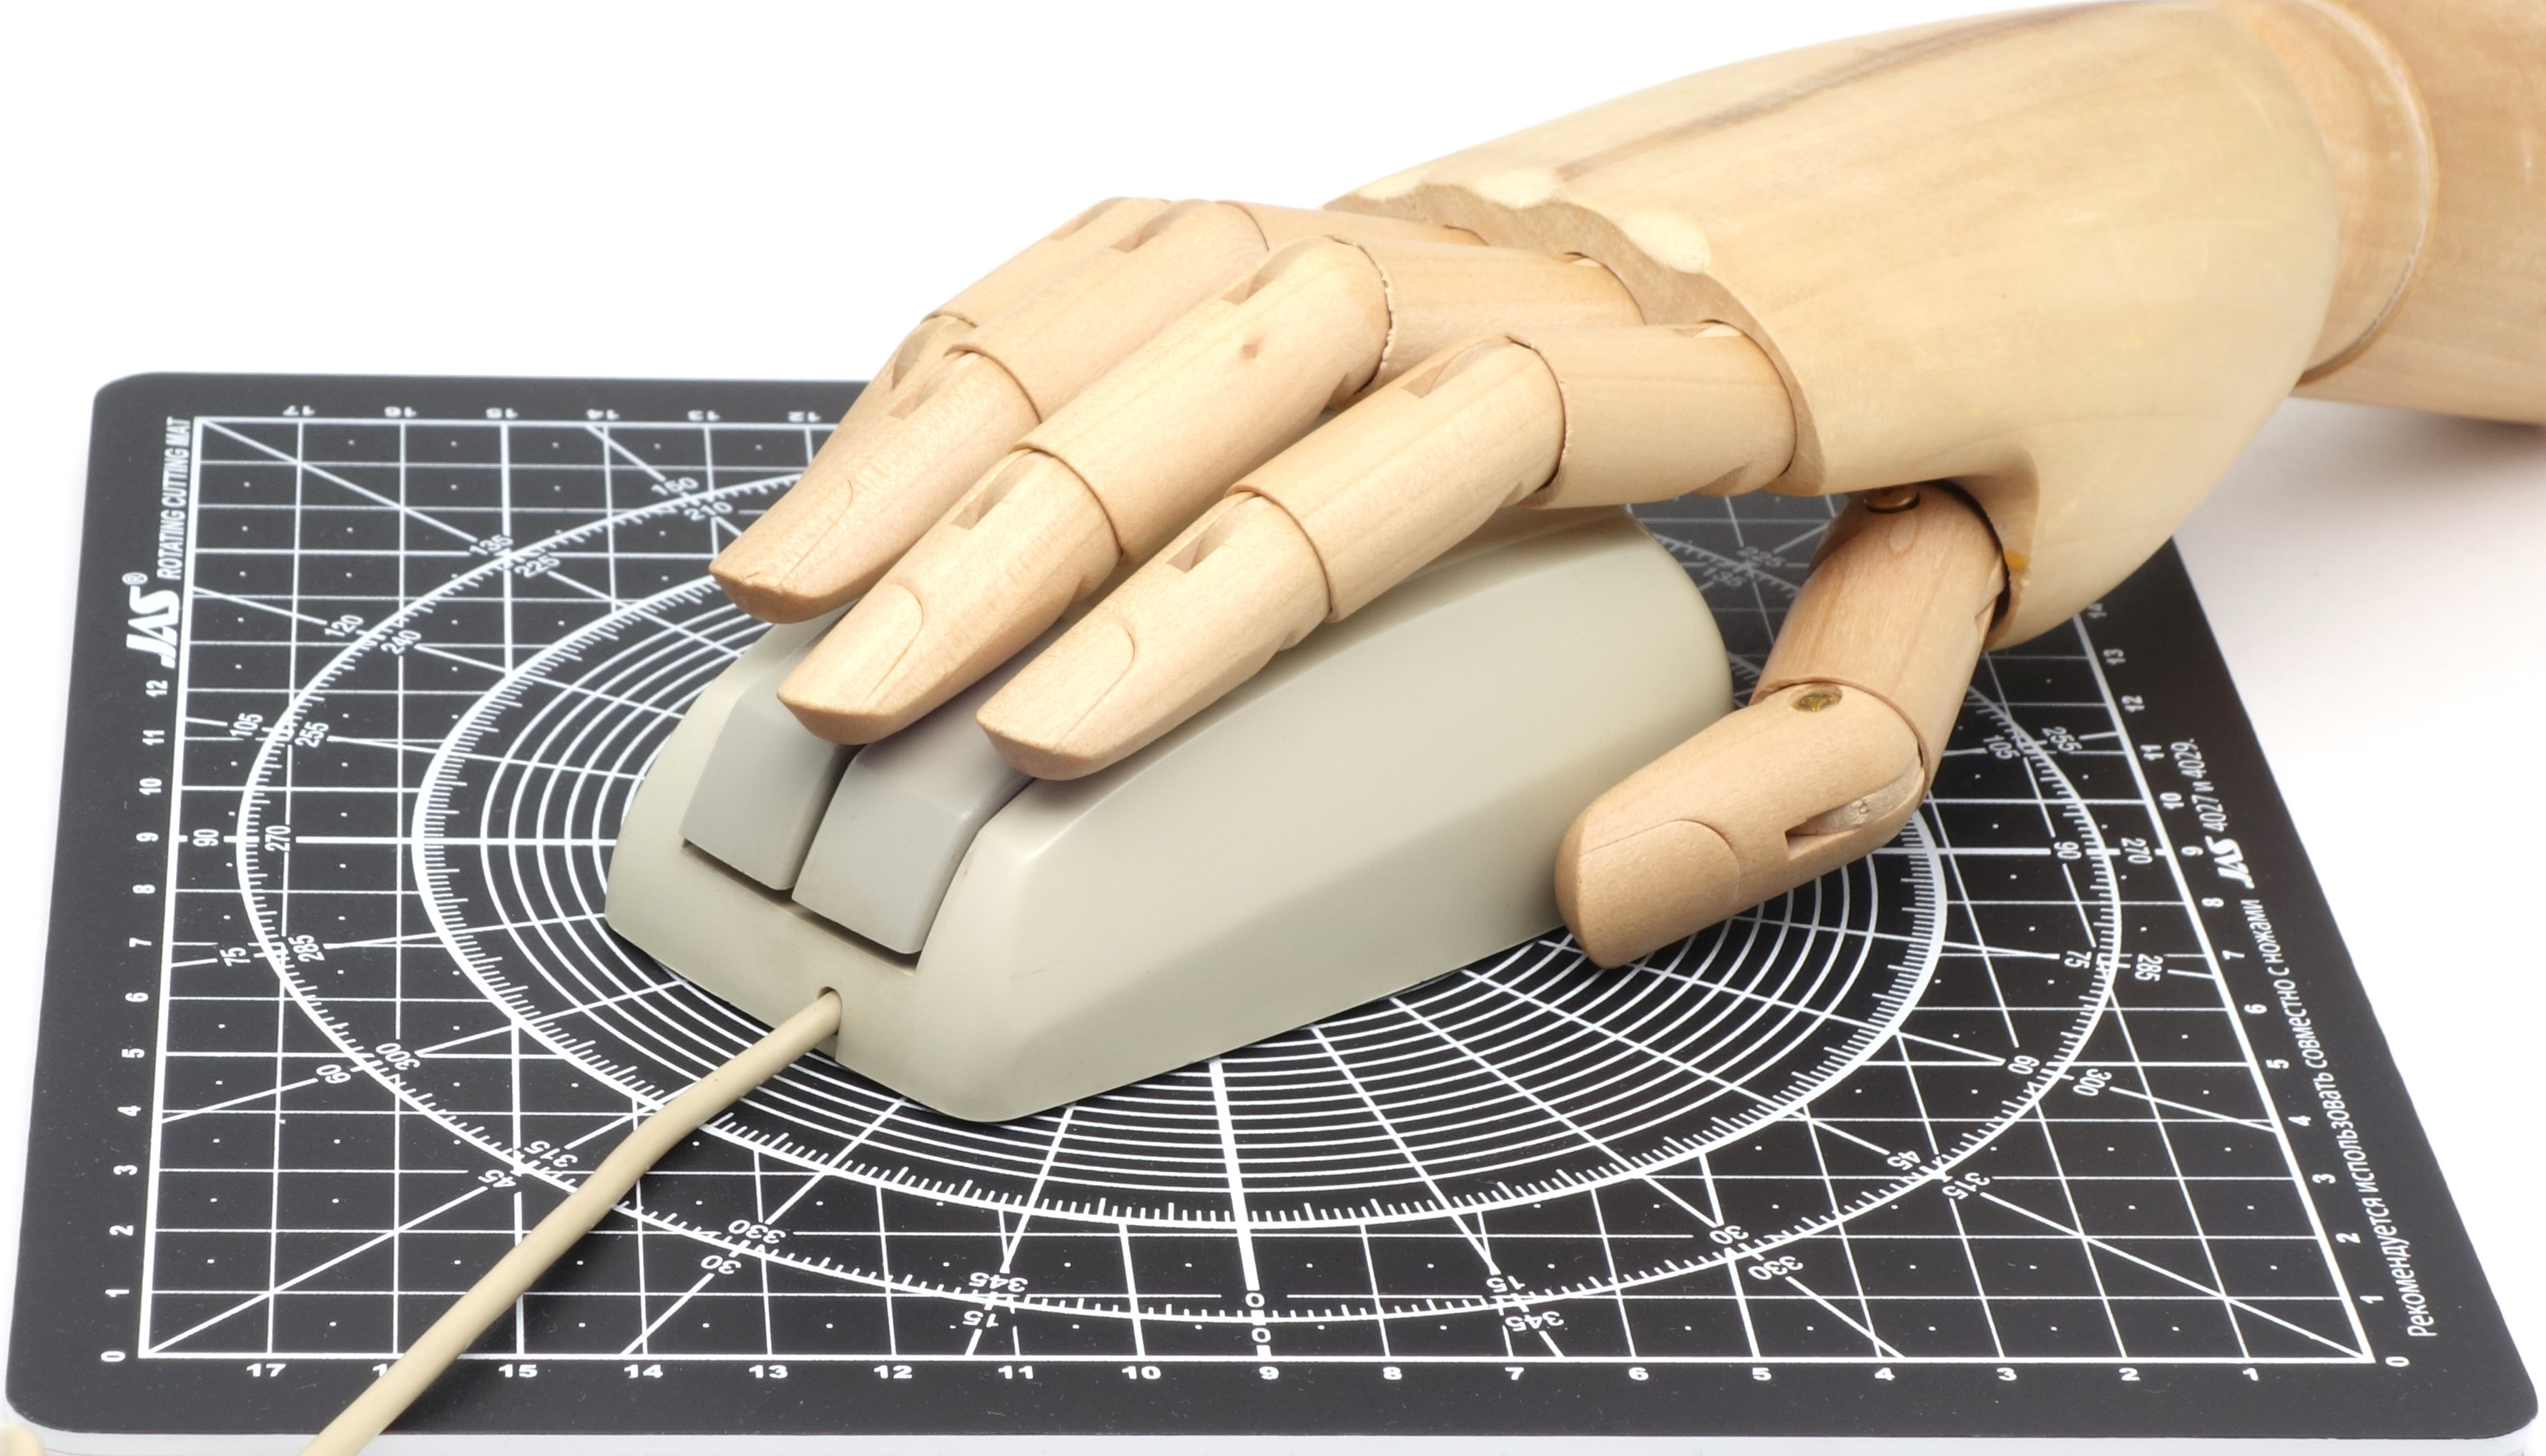
\includegraphics[scale=0.4]{1989_vatek_color_mouse/hand_30.jpg}
    \caption{Microsoft Gray-eyed Mouse с моделью руки человека}
    \label{fig:VatekColorHand}
\end{figure}

Color-Mouse подключается к компьютеру через последовательный порт с помощью 9-контактного разъема и имеет довольно умеренное разрешение "--- 250 точек на дюйм \cite{dpi}.

Изучение кода FCC ID по базе данных Федеральной комиссии по связи США показывает, что мышь была изготовлена компанией Jow Dian Enterprise Co Ltd., зарегистрированной в Калифорнии. Дата регистрации кода FCC ID "--- 1988 год, однако аналогичным кодом маркировалась и трехкнопочная мышь. Ранее выпуском двух поколений под одним кодом FCC ID отметилась Microsoft (самой первой <<зеленоглазой>> мыши и <<сероглазой>> мыши, у которой Jow Dian Enterprise позаимствовала форму корпуса). Сравнение маркировки печатных плат Color-Mouse и ProCorp Serial Mouse показывает, что Vatek Color-Mouse была второй ревизией. Поэтому, а также согласно \cite{mouses}, мышь датирована 1989 годом.

\begin{figure}[h]
    \centering
    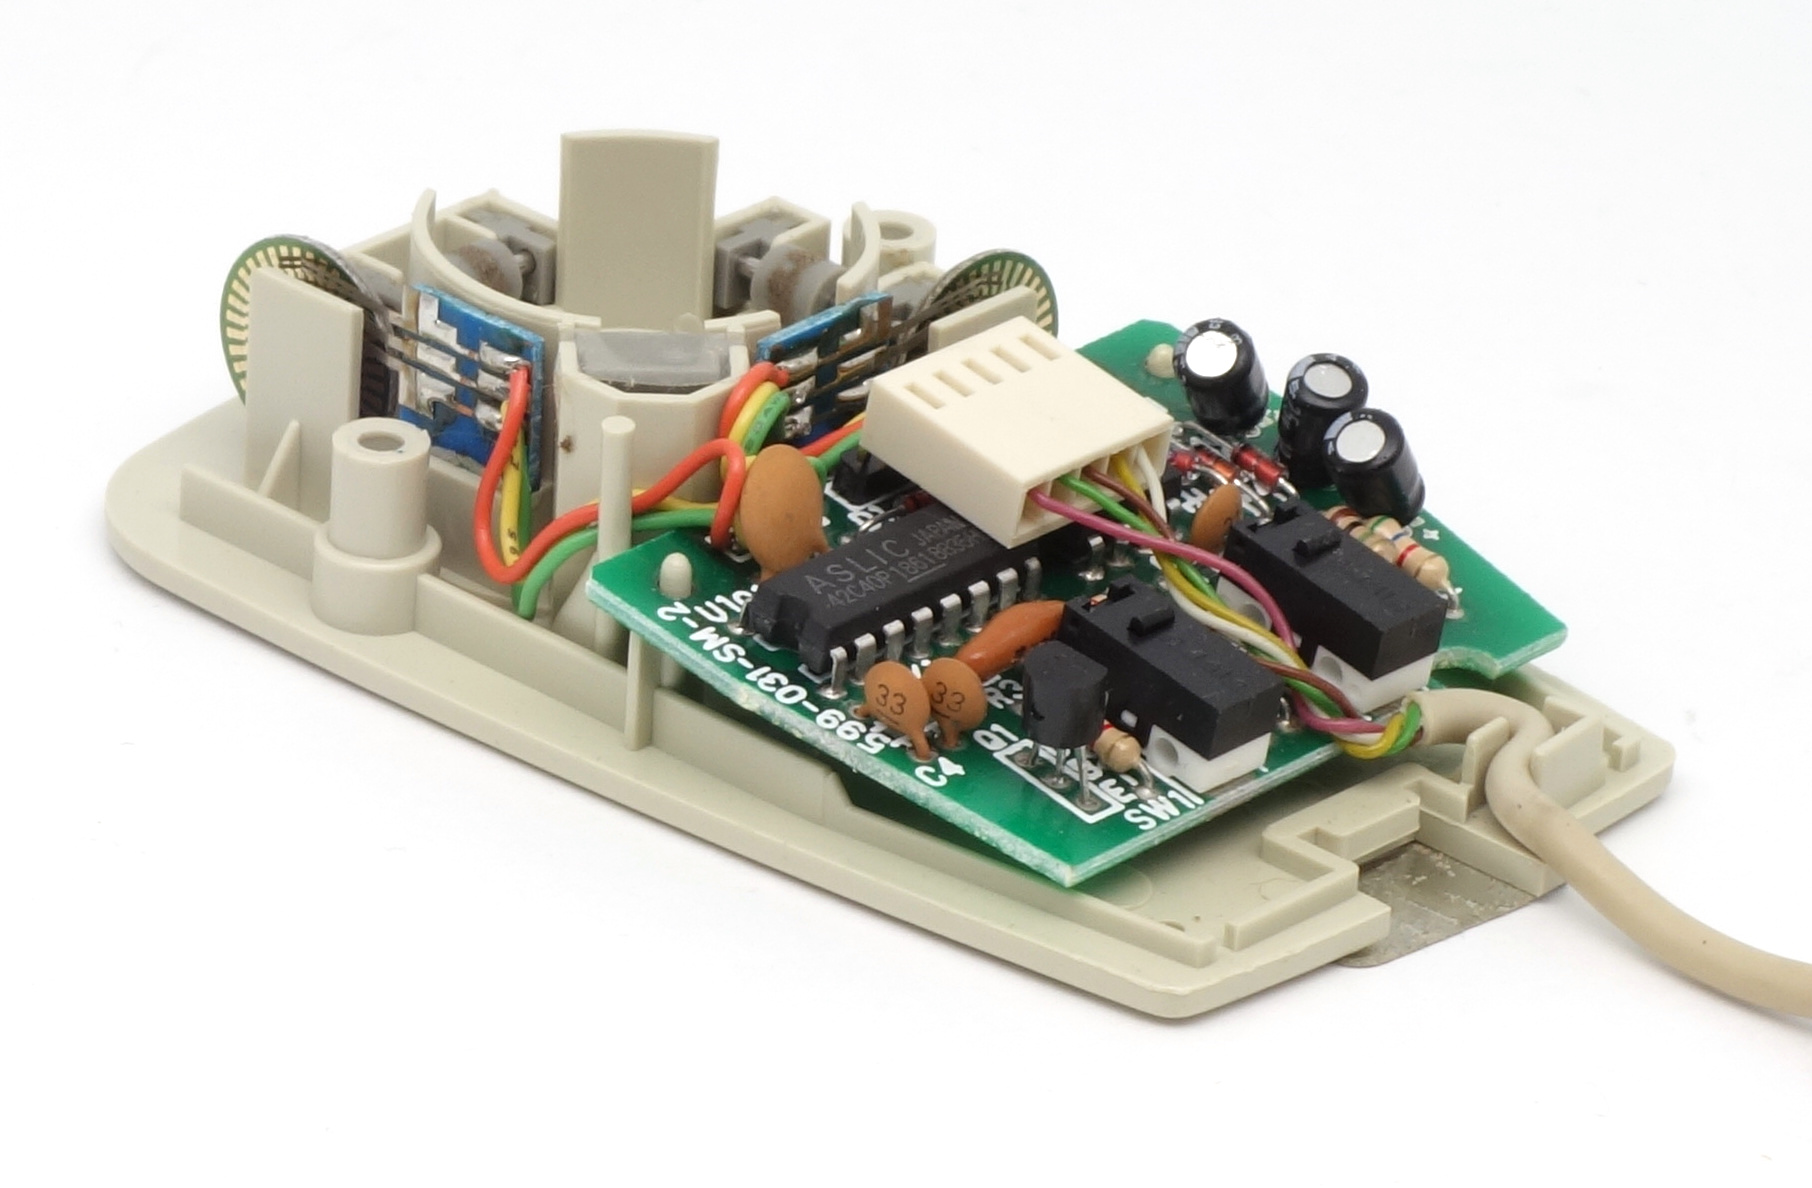
\includegraphics[scale=0.8]{1989_vatek_color_mouse/inside_60.jpg}
    \caption{Microsoft Gray-eyed Mouse в разобранном виде}
    \label{fig:VatekColorInside}
\end{figure}

Внутреннее устройство мыши показано на рис. \ref{fig:VatekColorInside}. По фотографии видно, что она является мышью с механическим энкодером, как и ее прототип от Microsoft, однако вместо более надежных закрытых энкодеров ALPS применен бюджетный вариант - открытый дисковый энкодер, встречающийся в мышах конца 80-х годов, чаще предназначенных для домашних компьютеров того времени, более простых и дешевых, чем IBM PC.

\begin{thebibliography}{9}
\bibitem{mouses} Vatek Color Mouse // Home Office Computing, December, 1989. -- P. 59 \url{https://forum.winworldpc.com/discussion/comment/152790/#Comment_152790}
\bibitem{company} Vatek USA * RMI Company Profile. \url{https://web.archive.org/web/19981201090808/http://www.vatek.com:80/company.html}
\bibitem{dpi} Color-Mouse // Dataquest: DQ, India: Cyber Media, 1990. p. 41.
\end{thebibliography}
\end{document}
